Figure \ref{fig:system_design} illustrates our general system design approach
that simulates the ecovisor infrastructure and integrates it into the Mosaik
co-simulation environment while enabling SIL capabilities. The present design
can be categorized into two distinct parts, the simulation of the ecovisor, and
its interface to external applications, which are elaborated on in the
following.

\begin{figure}
    \centering
    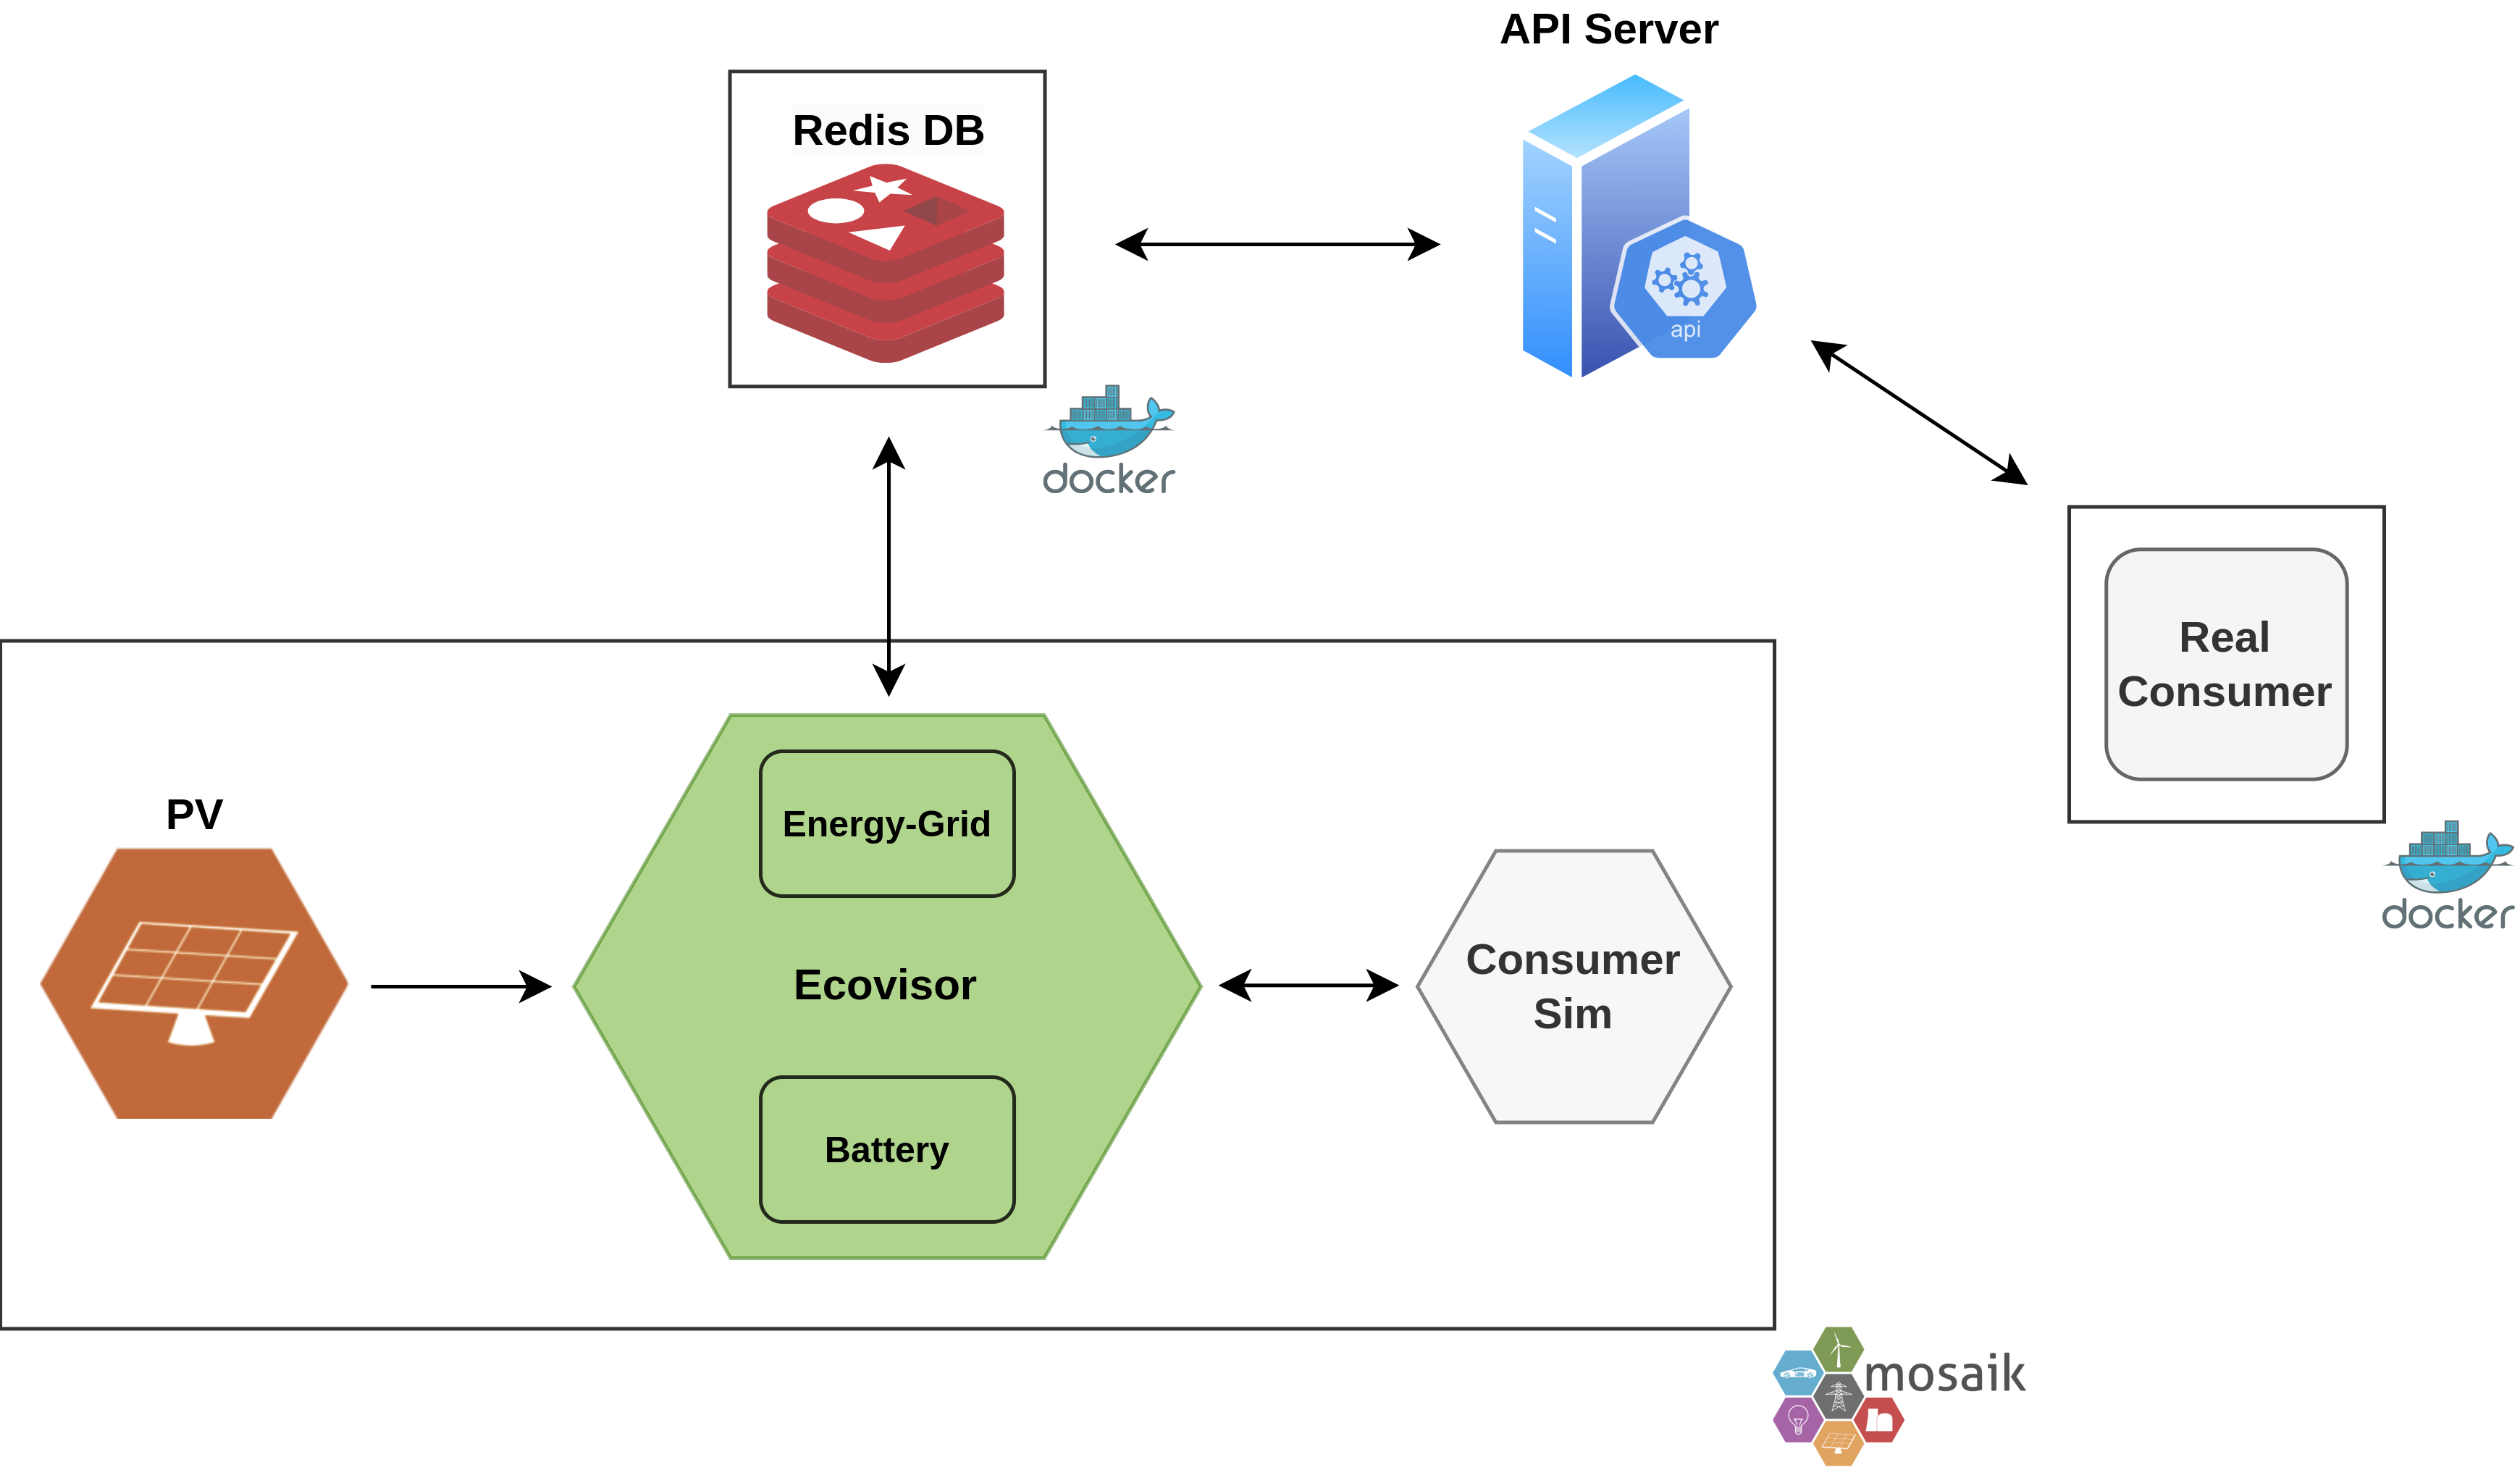
\includegraphics[width=\linewidth]{figures/system_design}
    \caption{
        General System Design: The ecovisor infrastructure is simulated and
        integrated into the Mosaik co-simulation environment. SIL capabilities
        are enabled via an API Server and a Redis database, connecting the
        simulation environment and real applications in real-time.
    }
    \label{fig:system_design}
\end{figure}

\subsection{Simulation of the Ecovisor}
The simulation part of our approach is fully contained within the Mosaik
co-simulation environment. In Figure \ref{fig:system_design} this includes the
photo-voltaic (PV) module, the ecovisor and a consumer simulator. The consumer
and PV module simulators utilized in this context are the \texttt{mosaik-csv}
simulator, which is a component of the Mosaik ecosystem \cite{mosaik_ecosystem}.
This simulator is capable of simulating CSV datasets, and in the current
application, it is employed to simulate consumption data and recorded or
forecasted PV data. While our primary focus is to facilitate the integration of
external, non-simulated applications with our simulated ecovisor, we also
recognize the need to accommodate simulated consumers for more sophisticated
approaches that require additional data. Therefore, we aim to provide
flexibility in our system to meet a wide range of requirements. Because these
two components are designed to be minimal and replaceable, they each require a
controller agent that acts as a medium between the component and the simulated
ecovisor. The controller can be initialized with e.g. a power conversion factor
to allow for the use of different measurement units in the datasets, as the
standard power unit utilized in the ecovisor is kW.

The simulated ecovisor holds all necessary variables to enable the API in Table
\ref{table:ecovisor_api}. This includes instances of a simple battery and
energy-grid model. The Simple Battery model can be configured with a capacity
and an initial charge. For every simulation step, the charge is incremented by
the delta value. The Simple Energy-Grid model reads carbon information from a
CSV dataset, either every simulation step line by line, or for a specific point
in time.

Because the co-simulation runs in real or \enquote{wall-clock} time, the Mosaik
scenario needs to be executed with \texttt{rt\_factor=1}. Most models in our
approach are time-based and one simulation step always translates to one second
in real-time in our environment. Therefore, we only model power as energy,
making the standard unit for our approach kWs instead of kW.

The simulation of the ecovisor's virtual energy system is realized in Algorithm
\ref{alg:virtual_energy_system_simulation}. Like its original counterpart, the
system prioritizes the utilization of virtual solar power to fulfill energy
requirements in line 1. The power values are centered around consumption.
Because solar power is \emph{adding} power to the system, its value is negative.
Therefore, if \texttt{rest} is negative or zero in line 2, there is extra solar
power and the battery does not discharge in line 3. In cases where solar power
is insufficient, the virtual energy system resorts to battery to compensate for
the shortfall in lines 5 -- 9. The discharge rate of the battery then depends on
its maximum discharge rate, the charge level of the battery and the power that
is attempted to be drawn. If the battery can not supply sufficient power, the
remaining power is being drawn from the grid in line 12. Lines 13 -- 15 then
adjust the battery's charge. Finally lines 16 -- 18 determine the carbon
concentration for the simulation step.

\begin{figure}
    \removelatexerror
    \begin{algorithm}[H]
        \caption{Virtual Energy System Simulation}
        \label{alg:virtual_energy_system_simulation}
        $rest \gets consumption - solar$\;
        \eIf{$rest \leq 0$} {
            \tcp{excess (or equal) solar power}
            $b\_discharge\_rate \gets 0$\;
        }{
            \tcp{solar power is insufficient \mbox{$\rightarrow$ use battery}}
            $b\_discharge\_rate \gets \text{min}($\;
            \Indp
                $b\_max\_discharge,$\;
                $b\_charge\_level \cdot 3600,$\;
                $rest$\;
            \Indm
            $)$\;
            $rest \gets rest - b\_discharge\_rate$\;
        }
        \tcp{draw remaining power from grid}
        $grid\_power \gets b\_charge\_rate + rest$\;
        \tcp{adjust battery charge}
        $b.delta \gets b\_charge\_rate - b\_discharge\_rate$\;
        $b.step()$\;
        $b\_charge\_level \gets b.charge$\;
        \tcp{determine carbon concentration for step}
        $energy\_grid.step()$\;
        $grid\_carbon \gets energy\_grid.carbon$\;
        $total\_carbon \gets grid\_carbon \cdot grid\_power$\;
        \vspace{3mm}
    \end{algorithm}
\end{figure}

Our approach does not implement a COP/Hypervisor. In the ecovisor, the COP
serves the primary purpose of granting containerized applications control over
their power consumption. Table \ref{table:ecovisor_api} shows that each
container can use the \texttt{set\_container\_powercap()} function to set their
power consumption limit. The ecovisor measures the power consumption of the
container using PowerAPI \cite{bourdon2013} and applies limits on resource
utilization using cgroups. The issue with PowerAPI is that it relies on
dedicated hardware equipped with sensors to collect raw data on software power
consumption. This collected data is then processed by a computational module
that utilizes a formula to \emph{estimate} the power consumption. A key
motivation behind the integration of the ecovisor into a co-simulation is to
create an affordable and accessible platform for researching and developing
carbon-aware applications. As power consumption measurement and control can vary
greatly depending on the research and development environment, we have chosen to
avoid implementing a specific strategy in order to allow for greater flexibility
and freedom.

\subsection{Interface to External Applications}

To integrate the ecovisor model with a real workload application, we exposed the
API as described in Table \ref{table:ecovisor_api} to containerized workloads.
This API was then integrated into a FastAPI server \cite{fastapi}. The API
server is connected to a Redis database \cite{redis}, which acts as a key-value
store and establishes a link between the API server and the ecovisor model. The
ecovisor model itself has been designed to implement a Redis interface that
enables it to read and write data from the RedisDB. In the following sections,
we will provide a detailed description of the three components that constitute
the External Application Interface.

\subsubsection{API-Server}

The ecovisor API is exposed to the workloads via the API-Server, which is
implemented using the FastAPI Framework and utilizes the Uvicorn web server
\cite{uvicorn} to handle multiple clients accessing the API. Since the web
server uses the ASGI (Asynchronous Server Gateway Interface) protocol, the
module is started as an independent thread. This allows the server to handle
multiple clients, which will be useful when multiple workloads are connected to
the simulation. However, implementing the module into the system was
challenging, so we decided to start it independently. In earlier versions, we
attempted to implement it inside the ecovisor model, but doing so halted the
execution of the simulation until the API-Server was stopped, rendering the
system unusable. Starting the API-Server independently also allows it to be
scaled independently from the ecovisor model and the RedisDB. This may be
helpful in bigger simulations with distributed infrastructure. We did not
implement the \textit{tick()} function from the ecovisor API since it is not
used in our approach, and Mosaic already includes a time mechanism for the
simulation part. Therefore, we have decided not to implement the \texttt{tick()}
endpoint to the API for now. However, we can easily add this functionality at a
later time.

\subsubsection{RedisDB}

The RedisDB is a high-speed, in-memory, key-value data store that is used in our
system to store and retrieve simple data types within the ecovisor model and
provide them to the API-Server. To simplify simulation operation, we start the
RedisDB as a Docker Container using the docker python library
\cite{docker_python}, which integrates the docker engine API into python. We use
the Redislabs Rejson Redis image \cite{RedisJSON}, which expands the RedisDB
image's functionality to handle JSON values. The Redis container is started at
the beginning of the simulation to ensure it is operational when the first data
is available. When the simulation ends, we stop and delete the container to keep
the test environment clean. The Ecovisor-Redis-Interface in the ecovisor model
can be adapted to replace the database with any other database, which may be
useful for integrating the simulation into a production-grade cloud environment
like Kubernetes or Openstack.

\begin{figure}
    \removelatexerror
    \begin{algorithm}[H]
        \caption{Energy Data JSON}
        \label{alg:energy_JSON}
        \{\;
        \Indp
            \enquote{solar\_power}: \enquote{0 kW},\;
            \enquote{grid\_power}: \enquote{0 kW},\;
            \enquote{grid\_carbon}: \enquote{0 g\,$\cdot$\,CO\textsubscript{2}/kW},\;
            \enquote{battery\_discharge\_rate}: \enquote{0 kW},\;
            \enquote{battery\_charge\_level}: \enquote{0 kWh}\;
        \Indm
        \}
        \vspace{3mm}
    \end{algorithm}
\end{figure}

\begin{figure}
    \removelatexerror
    \begin{algorithm}[H]
        \caption{Container Power Cap JSON}
        \label{alg:container_JSON}
        \{\;
        \Indp
            \enquote{Container\_ID 1}: \enquote{Power Cap 0 kW},\;
            \enquote{Container\_ID 2}: \enquote{Power Cap 0 kW},\;
            \enquote{Container\_ID n}: \enquote{Power Cap \dots}\;
        \Indm
        \}
        \vspace{3mm}
    \end{algorithm}
\end{figure}

\subsubsection{Ecovisor-Redis-Interface}

The interface to RedisDB is implemented within the ecovisor model using the
Redis-py library \cite{Redis-py} to simplify access. The ecovisor model has two
methods: \texttt{get\_redis\_updates()} and \texttt{send\_redis\_update()} which
are used to interact with RedisDB.

The \texttt{get\_redis\_update()} method is called at the beginning of the
\texttt{step()} method to update the simulation. This method is responsible for
updating the values of \texttt{battery\_discharge\_rate},
\texttt{battery\_charge\_level}, and \texttt{container\_power\_caps}. These
updated values are then used in subsequent power calculations within the
ecovisor model. To facilitate the exchange of data with the RedisDB, the data
structure presented in Algorithm \ref{alg:energy_JSON} is used. All the values
in this data structure are retrieved from the RedisDB, but only the values
mentioned above are updated and utilized in the simulation. Moreover, the data
structure \ref{alg:container_JSON} is employed to update the
\texttt{container\_power\_cap} of various workload applications. This process
helps to maintain the desired level of power consumption in the system and keep
it within the specified limits.

The \texttt{send\_redis\_updates()} method is called at the end of the
\texttt{step()} method, which publishes the updated values from the ecovisor
model. This includes data from other parts of the simulation that are accessible
by the ecovisor model. The data is exchanged with the RedisDB using the data
structure shown in Algorithm \ref{alg:energy_JSON}. Once the data is in RedisDB,
it can be accessed by the workload application via the API-Server.

\subsubsection{Dataflow}
\label{subsec:dataflow}
\begin{figure}
    \centering
    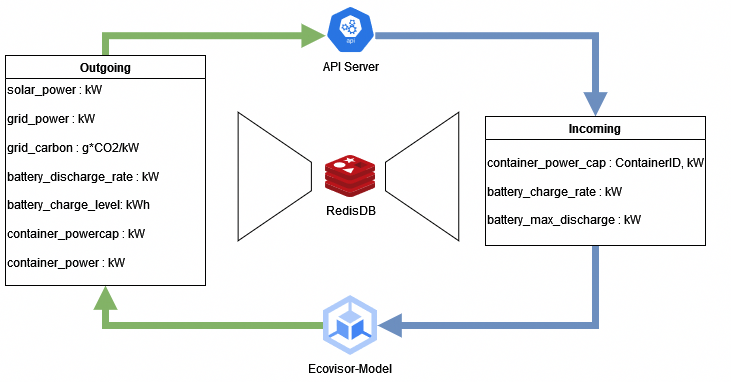
\includegraphics[width=\linewidth]{figures/Dataflow.drawio.png}
    \caption{Dataflow between ecovisor model and API Server}
    \label{fig:dataflow}
\end{figure}

In Figure \ref{fig:dataflow}, we can see the data exchange between the
API-Server and the ecovisor model, with two separate data streams: upstream from
the API-Server to the ecovisor model, and downstream from the ecovisor model to
the API-Server. The values written in each endpoint are not duplicated in the
other endpoint. The workload applications access the setter methods from Table
\ref{table:ecovisor_api}, which only affect the values
\texttt{container\_powercap}, \texttt{battery\_charge\_rate}, and
\texttt{battery\_max\_discharge}. These values are only read in the ecovisor
model. The values written by the ecovisor model are only accessible via the
getter-methods of the API. This setup ensures data consistency, since none of
the values can be written in parallel. Although the RedisDB theoretically
supports atomic writes to ensure data-consistency \cite{redis}, we do not
require this feature in our setup.

To model the entire data flow, the ecovisor model receives updates from the
RedisDB, processes the data, and sends the updated data back to the RedisDB so
that it can be accessed by the workload application. Any updates sent by the
workload application will be processed no later than the next call of the
\texttt{step()} method. This process encompasses the complete data flow between
the ecovisor model, the API server, and the workload applications.
